\documentclass[tikz,border=12pt]{standalone}
\usetikzlibrary{calc}
\begin{document}
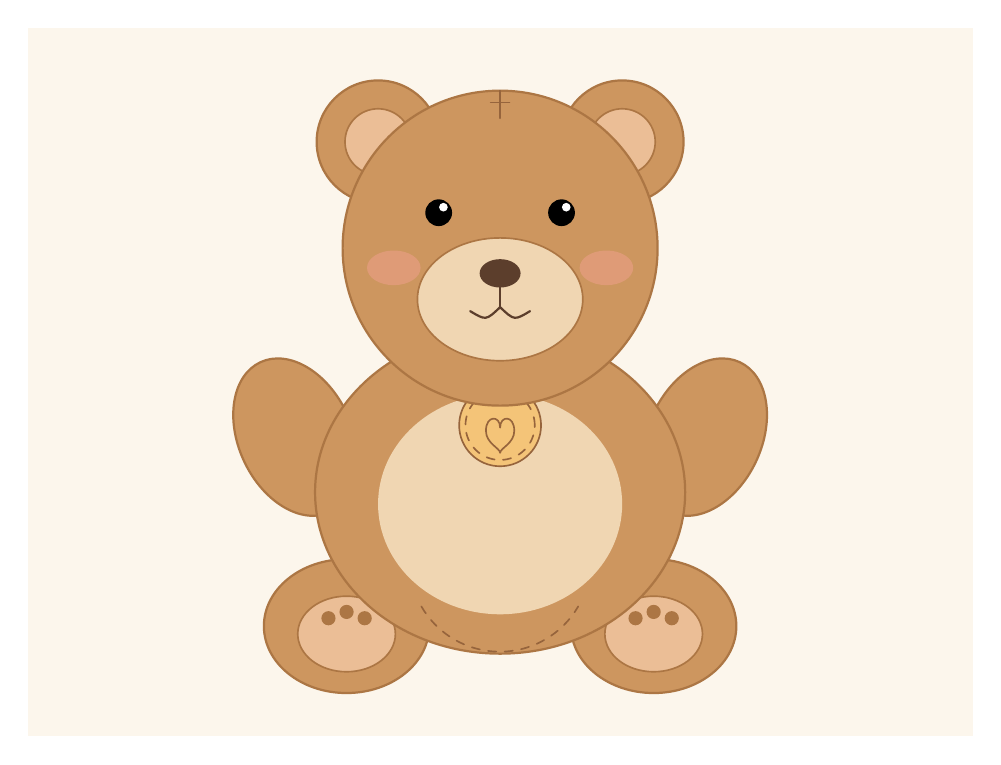
\begin{tikzpicture}[line cap=round,line join=round]
  \definecolor{fur}{RGB}{205,150,95}
  \definecolor{furdark}{RGB}{172,118,68}
  \definecolor{muzzle}{RGB}{240,214,178}
  \definecolor{pad}{RGB}{235,190,150}
  \definecolor{nose}{RGB}{92,62,44}
  \definecolor{patch}{RGB}{244,196,120}
  \definecolor{stitch}{RGB}{150,100,60}
  \definecolor{cheek}{RGB}{238,160,140}
  \definecolor{bgcard}{RGB}{252,246,236}

  % background card
  \fill[bgcard] (-6,-4.5) rectangle (6,4.5);

  % legs (short, rounded)
  \fill[fur,draw=furdark,thick] (-1.95,-3.1) ellipse (1.05 and 0.85);
  \fill[fur,draw=furdark,thick] (1.95,-3.1) ellipse (1.05 and 0.85);
  % foot pads
  \fill[pad,draw=furdark,semithick] (-1.95,-3.2) ellipse (0.62 and 0.48);
  \fill[pad,draw=furdark,semithick] (1.95,-3.2) ellipse (0.62 and 0.48);
  \fill[furdark] (-2.18,-3.0) circle (0.09) (-1.95,-2.92) circle (0.09) (-1.72,-3.0) circle (0.09);
  \fill[furdark] (1.72,-3.0) circle (0.09) (1.95,-2.92) circle (0.09) (2.18,-3.0) circle (0.09);

  % arms (short, rounded, slightly outward)
  \fill[fur,draw=furdark,thick,rotate around={25:(-2.6,-0.7)}] (-2.6,-0.7) ellipse (0.72 and 1.05);
  \fill[fur,draw=furdark,thick,rotate around={-25:(2.6,-0.7)}] (2.6,-0.7) ellipse (0.72 and 1.05);

  % body (soft, a bit wide)
  \fill[fur,draw=furdark,thick] (0,-1.4) ellipse (2.35 and 2.05);
  % belly
  \fill[muzzle] (0,-1.55) ellipse (1.55 and 1.4);
  % chest patch (heart-ish badge)
  \fill[patch,draw=stitch,semithick] (0,-0.55) circle (0.52);
  \draw[stitch,semithick] (-0.18,-0.62) .. controls (-0.18,-0.42) and (0,-0.42) .. (0,-0.58)
    .. controls (0,-0.42) and (0.18,-0.42) .. (0.18,-0.62)
    .. controls (0.18,-0.78) and (0,-0.84) .. (0,-0.9)
    .. controls (0,-0.84) and (-0.18,-0.78) .. (-0.18,-0.62);
  \draw[stitch,dashed,semithick] (0,-0.55) circle (0.44);

  % ears (symmetric, a bit large)
  \fill[fur,draw=furdark,thick] (-1.55,3.05) circle (0.78);
  \fill[fur,draw=furdark,thick] (1.55,3.05) circle (0.78);
  \fill[pad,draw=furdark,semithick] (-1.55,3.05) circle (0.42);
  \fill[pad,draw=furdark,semithick] (1.55,3.05) circle (0.42);

  % head (round)
  \fill[fur,draw=furdark,thick] (0,1.7) circle (2.0);

  % muzzle
  \fill[muzzle,draw=furdark,semithick] (0,1.05) ellipse (1.05 and 0.78);

  % eyes
  \fill[black] (-0.78,2.15) circle (0.17);
  \fill[black] (0.78,2.15) circle (0.17);
  \fill[white] (-0.72,2.22) circle (0.055);
  \fill[white] (0.84,2.22) circle (0.055);

  % cheeks
  \fill[cheek,opacity=0.55] (-1.35,1.45) ellipse (0.34 and 0.22);
  \fill[cheek,opacity=0.55] (1.35,1.45) ellipse (0.34 and 0.22);

  % nose and mouth
  \fill[nose] (0,1.38) ellipse (0.26 and 0.18);
  \draw[nose,thick] (0,1.2) -- (0,0.95);
  \draw[nose,thick] (0,0.95) .. controls (-0.18,0.78) .. (-0.38,0.9);
  \draw[nose,thick] (0,0.95) .. controls (0.18,0.78) .. (0.38,0.9);

  % stitches for plush texture
  \draw[stitch,semithick] (0,3.7) -- (0,3.35);
  \draw[stitch,semithick] (-0.12,3.55) -- (0.12,3.55);
  \draw[stitch,dashed,semithick] (-1.0,-2.85) arc[start angle=210,end angle=330,radius=1.15];
\end{tikzpicture}
\end{document}
